\documentclass[11pt]{article}
%\documentclass[12pt]{article}
%\documentclass[12pt]{article}
%\documentclass[12pt,a4paper]{article}

\usepackage[percent]{overpic}
\usepackage{float}
\usepackage{pgfplots}
%\usepackage[cmbold]{mathtime}
%\usepackage{mt11p}
\usepackage{placeins}
\usepackage{amsmath}
\usepackage{amsthm}
\usepackage{color}
\usepackage{amssymb}
\usepackage{mathtools}
\usepackage{subfigure}
\usepackage{multirow}
\usepackage{epsfig}
\usepackage{listings}
\usepackage{enumitem}
\usepackage{rotating,tabularx}
%\usepackage[graphicx]{realboxes}
\usepackage{graphicx}
\usepackage{graphics}
\usepackage{epstopdf}
\usepackage{longtable}
\usepackage[pdftex]{hyperref}
%\usepackage{breakurl}
\usepackage{epigraph}
\usepackage{xspace}
\usepackage{amsfonts}
\usepackage{eurosym}
\usepackage{ulem}
\usepackage{footmisc}
\usepackage{comment}
\usepackage{setspace}
\usepackage{geometry}
\usepackage{caption}
\usepackage{pdflscape}
\usepackage{array}
\usepackage[round]{natbib}
\usepackage{booktabs}
\usepackage{dcolumn}
\usepackage{mathrsfs}
%\usepackage[justification=centering]{caption}
%\captionsetup[table]{format=plain,labelformat=simple,labelsep=period,singlelinecheck=true}%

%\bibliographystyle{unsrtnat}
\bibliographystyle{aea}
\usepackage{enumitem}
\usepackage{tikz}
\usetikzlibrary{decorations.pathreplacing}
%\def\checkmark{\tikz\fill[scale=0.4](0,.35) -- (.25,0) -- (1,.7) -- (.25,.15) -- cycle;}
%\usepackage{tikz}
%\usetikzlibrary{snakes}
%\usetikzlibrary{patterns}

%\draftSpacing{1.5}

\usepackage{xcolor}
\hypersetup{
colorlinks,
linkcolor={blue!50!black},
citecolor={blue!50!black},
urlcolor={blue!50!black}}

%\renewcommand{\familydefault}{\sfdefault}
%\usepackage{helvet}
%\setlength{\parindent}{0.4cm}
%\setlength{\parindent}{2em}
%\setlength{\parskip}{1em}

%\normalem

%\doublespacing
\onehalfspacing
%\singlespacing
%\linespread{1.5}

\newtheorem{theorem}{Theorem}
\newcommand{\bc}{\begin{center}}
\newcommand{\ec}{\end{center}}
\newtheorem{corollary}[theorem]{Corollary}
\newtheorem{proposition}{Proposition}
\newtheorem{definition}{Definition}
\newtheorem{axiom}{Axiom}
\newcommand{\ra}[1]{\renewcommand{\arraystretch}{#1}}

\newcommand{\E}{\mathrm{E}}
\newcommand{\Var}{\mathrm{Var}}
\newcommand{\Corr}{\mathrm{Corr}}
\newcommand{\Cov}{\mathrm{Cov}}

\newcolumntype{d}[1]{D{.}{.}{#1}} % "decimal" column type
\renewcommand{\ast}{{}^{\textstyle *}} % for raised "asterisks"

\newtheorem{hyp}{Hypothesis}
\newtheorem{subhyp}{Hypothesis}[hyp]
\renewcommand{\thesubhyp}{\thehyp\alph{subhyp}}

\newcommand{\red}[1]{{\color{red} #1}}
\newcommand{\blue}[1]{{\color{blue} #1}}

%\newcommand*{\qed}{\hfill\ensuremath{\blacksquare}}%

\newcolumntype{L}[1]{>{\raggedright\let\newline\\arraybackslash\hspace{0pt}}m{#1}}
\newcolumntype{C}[1]{>{\centering\let\newline\\arraybackslash\hspace{0pt}}m{#1}}
\newcolumntype{R}[1]{>{\raggedleft\let\newline\\arraybackslash\hspace{0pt}}m{#1}}

%\geometry{left=1.25in,right=1.25in,top=1.25in,bottom=1.25in}
\geometry{left=1in,right=1in,top=1in,bottom=1in}

\epstopdfsetup{outdir=./}

\newcommand{\elabel}[1]{\label{eq:#1}}
\newcommand{\eref}[1]{Eq.~(\ref{eq:#1})}
\newcommand{\ceref}[2]{(\ref{eq:#1}#2)}
\newcommand{\Eref}[1]{Equation~(\ref{eq:#1})}
\newcommand{\erefs}[2]{Eqs.~(\ref{eq:#1}--\ref{eq:#2})}

\newcommand{\Sref}[1]{Section~\ref{sec:#1}}
\newcommand{\sref}[1]{Sec.~\ref{sec:#1}}

\newcommand{\Pref}[1]{Proposition~\ref{prop:#1}}
\newcommand{\pref}[1]{Prop.~\ref{prop:#1}}
\newcommand{\preflong}[1]{proposition~\ref{prop:#1}}

\newcommand{\Aref}[1]{Axiom~\ref{ax:#1}}
\newcommand{\Dref}[1]{Definition~\ref{def:#1}}

\newcommand{\clabel}[1]{\label{coro:#1}}
\newcommand{\Cref}[1]{Corollary~\ref{coro:#1}}
\newcommand{\cref}[1]{Cor.~\ref{coro:#1}}
\newcommand{\creflong}[1]{corollary~\ref{coro:#1}}

\newcommand{\etal}{{\it et~al.}\xspace}
\newcommand{\ie}{{\it i.e.}\xspace}
\newcommand{\eg}{{\it e.g.}\xspace}
\newcommand{\etc}{{\it etc.}\xspace}
\newcommand{\cf}{{\it c.f.}\xspace}
\newcommand{\ave}[1]{\left\langle#1 \right\rangle}
\newcommand{\person}[1]{{\it \sc #1}}

\newcommand{\AAA}[1]{\red{{\it AA: #1 AA}}}
\newcommand{\YB}[1]{\blue{{\it YB: #1 YB}}}

\newcommand{\flabel}[1]{\label{fig:#1}}
\newcommand{\fref}[1]{Fig.~\ref{fig:#1}}
\newcommand{\Fref}[1]{Figure~\ref{fig:#1}}

\newcommand{\tlabel}[1]{\label{tab:#1}}
\newcommand{\tref}[1]{Tab.~\ref{tab:#1}}
\newcommand{\Tref}[1]{Table~\ref{tab:#1}}

\newcommand{\be}{\begin{equation}}
\newcommand{\ee}{\end{equation}}
\newcommand{\bea}{\begin{eqnarray}}
\newcommand{\eea}{\end{eqnarray}}
\newcommand{\bi}{\begin{itemize}}
\newcommand{\ei}{\end{itemize}}
\newcommand{\Dt}{\Delta t}
\newcommand{\Dx}{\Delta x}
\newcommand{\Epsilon}{\mathcal{E}}
\newcommand{\etau}{\tau^\text{eqm}}
\newcommand{\wtau}{\widetilde{\tau}}
\newcommand{\xN}{\ave{x}_N}
\newcommand{\Sdata}{S^{\text{data}}}
\newcommand{\Smodel}{S^{\text{model}}}
\newcommand{\subhead}[1]{\mbox{}\newline\textbf{#1}\newline}
\setlength{\parindent}{0.0cm}
\setlength{\parskip}{0.4em}
\numberwithin{equation}{section}
\DeclareMathOperator\erf{erf}
%\let\endtitlepage\relax
\begin{document}
\begin{titlepage}
\title{Mobility, Mixing and Ergodicity: A Physically-Motivated Measure for Economic Mobility}
\author{Viktor Stojkoski\footnote{Macedonian Academy of Sciences and Arts,~\url{vstojkoski@manu.edu.mk}} \and Alexander Adamou\footnote{London Mathematical Laboratory,~\url{a.adamou@lml.org.uk}} \and Yonatan Berman\footnote{London Mathematical Laboratory,~\url{y.berman@lml.org.uk}} \and Colm Connaughton\footnote{London Mathematical Laboratory and University of Warwick,~\url{c.p.connaughton@warwick.ac.uk}} \and Ole Peters\footnote{London Mathematical Laboratory and Santa Fe Institute,~\url{o.peters@lml.org.uk}}\,\, \thanks{We thank...}}
%\date{First version: August 26, 2018\,\,\,\,\,\,\,\,\,\,\,\,\,\,\,\,\,\,\,\,\,\,\,\,Last revised: \today}
%\date{}
\date{\today}
\maketitle
%\bc
%\red{Preliminary version, please do not circulate}
%\ec
\begin{abstract}
\noindent Standard measures of economic mobility do not account for the possible non-ergodic income or wealth dynamics. Thus, they may not provide an adequate picture of mobility within an economy. Here we introduce mixing time as a measure of economic mobility. Mixing time quantifies the characteristic time scale over which individual incomes or wealths mix into the distribution. By construction, it is finite only in an ergodic system and then there is a direct equivalence between its value and the magnitude of the standard measures of economic mobility. On the other hand, the opposite is not true. Hence, measuring mobility using standard measures in a non-ergodic system may be misleading. We display the properties of mixing time by studying mobility in reallocating geometric Brownian motion -- an established model of wealth in a growing and reallocating economy.
\\

\noindent\textbf{Keywords: mobility, inequality, ergodicity economics}
%\\
%\bigskip
\end{abstract}
\setcounter{page}{0}
\thispagestyle{empty}
%\nopagebreak
\end{titlepage}
\pagebreak \newpage
%\nopagebreak
\section{Introduction}\label{sec:introduction}
% What is mobility?
Economic mobility describes ``dynamic aspects of inequality'' \citep{Shorrocks1978}. It quantifies how wealth (or income\footnote{We focus on wealth in this paper, but our findings also apply to income}) ranks of individuals change over time. Intuitively, when mobility is high, ranks evolve quickly, and the chances of an individual to change her position in the wealth distribution over a given time period are high. When mobility is low, individuals are unlikely to change their rank in the distribution over time, or that it changes slowly.

% How is mobility typically measured?
\citet{Shorrocks1978} described several required properties of statistical measures of mobility and set the standard for such measures. Mobility measures are assumed to be derived from the joint distribution of wealth at two points in time.
%The joint distribution of wealth ranks can be described using a transition matrix, describing the conditional probabilities of individuals to move between different ranks over some time period.
An example for such a measure, used extensively in the mobility literature, is the rank correlation, the correlation between individual wealth ranks at two points in time. Another canonical measure of mobility, used most typically in studies of intergenerational income mobility, is the intergenerational earnings elasticity (IGE), defined as the regression coefficient between log-incomes of parents and children.\footnote{In fact, the rank correlation and the IGE are both measures of immobility, and to consider them as measures of mobility one has to consider their complement or their inverse.}

% Why are the typical measures problematic?
The standard statistical measures of mobility have several limitations. First, they are generally incomparable. For example, a rank correlation of 0.3 would have a different meaning if it corresponds to a period of one year or ten years. Second, for a given time period, it is not possible to tell whether some value of rank correlation is high or low, as this is a dimensionless quantity. Thus, the rank correlation over some time period can only be high or low in comparison to other economies over a similar time period, or to other time periods of the same length.

In addition, the interpretation of the rank correlation depends on the underlying wealth distribution and its dynamics. The same rank correlation cannot be interpreted similarly when the underlying wealth distribution remains unchanged, and when it becomes more and more unequal. The IGE has similar limitations, but also others. Most notably, the IGE is sensitive by design to the level of inequality and not only to the transition matrix, as discussed in detail in the mobility literature (\eg \citet{chettyETAL2014}).

% This paper
This paper introduces mixing time, a property of dynamical systems, as a measure of mobility. When wealth is an ergodic observable \citep{PetersAdamou2018c}, and assuming the wealth distribution approaches a steady state, if the wealths of an arbitrary group of individuals is followed over time, the distribution of wealth within this group will gradually become similar to the steady-state wealth distribution. The characteristic time of this convergence process is the mixing time. Put simply, it is the time scale over which individuals mix into the wealth distribution. When mixing is rapid, \ie the mixing time is short relative to the window of observation, we could interpret that as high wealth mobility. Slow mixing is interpreted as low mobility.

% We study RGBM
We then consider Reallocating Geometric Brownian Motion (RGBM \citep{MarsiliMaslovZhang1998,LiuSerota2017,BermanPetersAdamou2019}) as a model for wealth dynamics and study mixing in this model. In RGBM, individual wealth undergoes random multiplicative growth, modeled as Geometric Brownian Motion (GBM), and is reallocated among individuals by a simple pooling and sharing mechanism. RGBM is a null model of an exponentially growing economy with social structure. It has three parameters representing economic growth, random shocks to individual wealth, and economic interaction among agents, quantified by the reallocation rate. This model is known to reproduce several important stylized facts. In particular, when the reallocation rate is positive, the wealth distribution converges to a stationary distribution with a Pareto tail. The model has both ergodic and non-ergodic regimes, characterized by the sign of the reallocation rate parameter \citep{BermanPetersAdamou2019}.

% What is the mixing time in RGBM?
We find that in the ergodic regime of RGBM the mixing time scales with the inverse of the reallocation rate. As the reallocation rate becomes higher, \ie when a larger share of each individual's wealth is pooled and then shared per unit time, mixing time becomes shorter proportionally, and mobility increases. As the reallocation rate approaches zero, mixing times get longer, and mobility lower. Since decreasing reallocation rates also lead to increasing inequality, this result is in line with the empirical observation that as inequality increases mobility decreases, and vice versa \citep{corak2013}. There is also a direct relationship between mixing time and standard measures of economic mobility. The intragenerational copulas produced by RGBM closely resemble Gumbel copulas \citep{Gumbel1958,TrivediZimmer2007}, often used in the mobility literature.

% Mixing in non-ergodic systems
In practice, however, many economic systems are best modeled as non-ergodic \citep{Peters2019b}. In particular, \citet{BermanPetersAdamou2019} argue that the US economy is best described in RGBM as one in which wealth is systematically reallocated from poorer to richer, \ie the reallocation rate is negative. In this case, even though the standard measures of economic mobility might suggest existence of mobility, there is no mixing, so the mixing time is infinite. Thus, measuring mobility using standard measures under this regime may be misleading. The thorough study of RGBM in this regime is outside of the scope of this paper and left for future work.

% Plan
The paper is organized as follows. In~\Sref{standard-measures} we present some limitations of the standard measures of economic mobility.~\Sref{mixing-time} discusses the concept of mixing time and how it provides a physically-motivated measure for mobility.~\Sref{rgbm} studies mobility using mixing times in reallocating geometric Brownian motion as a model for wealth. We discuss our findings in~\Sref{discussion}.

\section{Standard measures of economic mobility and their limitations}\label{sec:standard-measures}

We begin with an overview of two standard measures of economic mobility: Spearman's rank correlation and the intergenerational elasticity (IGE). These measures describe properties of the bivariate joint wealth distribution in two points in time. We also consider the transition matrix, or copula, from which various mobility measures can be derived.\footnote{Technical background is given in Appendix~\ref{sec:standard-mobility-measures}.}

Our focus here is on limitations and caveats in these measures. We visualize some limitations in \fref{standard-mobility-measures}, in which we construct a simplified example in economy with 9 individuals, during 3 time periods. At the left panel we show the dynamics of the wealth ranks. We also highlight the amount of wealth owned by a person with a colored circle, with darker colored and larger circle implying a wealthier person.

\begin{figure}[!htb]
\centering
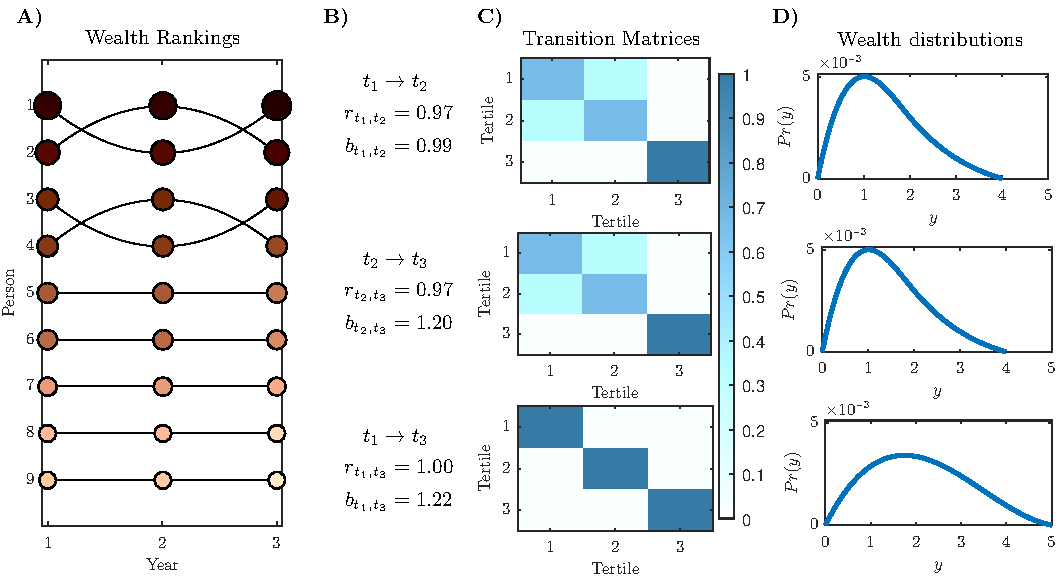
\includegraphics[width=1.0\textwidth]{figs/fig_mobility_measures.pdf}
\caption{\textbf{Mobility measures in a simplified example.} \textbf{A)} Dynamics of the wealth rankings in a simplified economy consisting of 9 individuals, during 3 time periods. \textbf{B)} Estimated Spearman's rank correlation and IGE during the studied periods. \textbf{C)} The corresponding mobility transition matrices. \textbf{D)} The distribution of wealth $x(t)$ for the 3 time periods.
\label{fig:standard-mobility-measures}}
\end{figure}

In our example only the four richest individuals changed their wealth rank. In particular, in the second period, $t_2$, the second richest person becomes the richest, while the richest person in the first period $t_1$ becomes second richest. In addition, the third and fourth richest individuals also switch their positions. In period $t_3$, the dynamics are reversed, thus ending up with the same wealth rankings as in $t_1$. The only difference is that in this period, the distribution of wealth has changed, with the richest individual being richer than in the previous periods.

If we were to look at the rank correlation, it shows that mobility was the same between $t_1$ and $t_2$, and between $t_2$ and $t_3$. However, overall, between $t_1$ and $t_3$ it would show no mobility ($r_{t_1,t_3} = 1$). As inequality increased in the last period, the IGE suggests that the economy became less mobile.

The same conclusions hold when looking at the transition matrices estimated by dividing the wealth rankings into tertiles. The transition matrices between $t_1$ and $t_2$ and between $t_2$ and $t_3$ suggest that there is a $p=1/3$ probability for an individual in the second tertile to climb up to the richest tertile and vice versa. Yet, we structured our economy in a way that allows movement only between the individuals at the edge of the tertile, so the transition matrices fail to adequately represent the movement of the typical person in the tertile.

This example shows that standard measures of economic mobility represent aggregate values of the changes in the wealth rankings of the individuals which constitute the population between two time periods. Therefore, they rely on a relevant time period over which the wealth rankings are compared. A rank correlation of 0.3 would have a different meaning if it corresponds to a period of one year or ten years. Also, for a given time period, it is not possible to tell whether some value of rank correlation is high or low, as this is a dimensionless quantity. Thus, rank correlation over some time period can only be high or low in comparison to other economies over a similar time period, or to other time periods of the same length.

The standard measures do not quantify the mobility of the typical representative of the population. In our simplified economy the bottom tertile is perfectly immobile. Regardless of the rank correlation value, it is not representative of the dynamics of wealth of individuals belonging to this tertile. In addition, quantifying mobility using the transition matrix (and deriving various functionals of it as mobility indicators), implicitly assumes the Markov property -- that if transition matrix $\mathbf{A}$ represents the period between $t_1$ and $t_2$ and $\mathbf{B}$ the period between $t_2$ and $t_3$, then $\mathbf{A B}$ would represent the transition matrix between $t_1$ and $t_3$. This is not inline with empirical findings \citep{Mcfarland1970,Shorrocks1978,Clark2015}.

\FloatBarrier
\section{Mixing time as a measure of mobility}
\label{sec:mixing-time}

The concept of mixing time comes from probability theory and statistical physics. It allows overcoming the limitations discussed above. A mixing time would provide a characteristic time scale over which individuals mix into the wealth distribution. Figuratively, we can think of the economy as a cup of coffee and of some person's wealth as milk poured in the coffee. The mixing time quantifies the time required for the milk to blend with the coffee. This enables the measure to be used for appropriate comparison between different time periods and economies.

As we will see in the following sections, there is a relationship between the mixing time and standard mobility measures, whenever mixing time is a finite quantity. However, the standard measures may still indicate that there is some level of mobility even when mixing does not occur (\ie the mixing time is infinite). This is because mixing time depends on the existence of mobility between \textit{every} quantile in the wealth distribution. In other words, finite mixing times require wealth to be ergodic, and we will argue that in the absence of ergodicity, mobility cannot be properly defined.\footnote{This idea was already described by \citet{Mcfarland1970}.}

\subsection{Measuring mixing times}

In physical terms, mixing describes the property of a dynamical system being strongly intertwined. That is, in any set of particles in a dynamical system the fraction of the particles found within a particular region in the \textit{phase space} (the space of the variable $x$ characterizing the particles, wealth in our case), is proportional to the volume of that region in the phase space. If the system is mixing this occurs after a sufficient period of time, the mixing time, regardless of the particles' initial condition.

%Mixing is strongly related to the concept of ergodicity. However, the latter is a broader concept: An observable $x$ is said to be ergodic if its time-average is to its ensemble averages at any given time. Put differently, ergodicity implies that every trajectory moves around the phase space over time according to the steady state distribution of $x$. Hence, every dynamical system that is mixing is also ergodic, but the opposite is not necessarily true.

In economic terms, mixing implies that there always exists a stationary distribution to which some rescaled transformation of a person's wealth converges. It further indicates that mobility between every possible quantile in the population exists. The mixing time gives an estimate for the relevant time scale for this kind of mobility to occur.

Using mixing times overcomes the limitations of the standard measures in several ways. First, the mixing time is measured in units of time. This means that when mixing is rapid, \ie the mixing time is short relative to a relevant window of observation, we could interpret that as high wealth mobility. Slow mixing is interpreted as low mobility. This overcomes the necessity to define high or low mobility with respect to other countries or to the past. Second, the mixing time is a finite quantity only when each individual is able to move across the whole distribution of wealth. Therefore, it does not represent an aggregate measure of the mobility in the economy. It captures the feasibility of \textit{all} individuals to change their wealth status.

The described properties of a mixing economy can also be utilized to develop an estimation procedure for mixing time. The first step is defining a relevant steady state distribution to which the rescaled transformation of wealth converges. We then select any subsample of the population and track their wealth, following the subsample wealth distribution over time, and quantify the difference between the subsample wealth distribution and the steady state distribution with a distance measure (\eg the Kolmogorov-Smirnov statistic). In a mixing economy the statistic will exhibit two states. First, there will be a mixing time state during which the two distributions will converge towards each other, and the statistic will decrease. After a transitory phase, there will be a stable state. In the stable state the log of the statistic reaches a plateau and fluctuate around this plateau. The magnitude of the plateau will be determined by the subsample size: smaller sample sizes will exhibit higher plateau and vice versa. This is a finite sample size effect. The last step is to utilize the data only for the mixing time state and regress the log of the statistic on time. The mixing time is the additive inverse of the reciprocal value of the slope ($-1/slope$).

\Fref{mixing-time} summarizes the procedure. The blue line is the log of an arbitrary distance statistic such as the Kolmogorov-Smirnov as a function of time. The dashed black line is a regression line for the relationship between the statistic and time during the two different states. The inset plots provide snapshots for the wealth distribution of the subsample at different time points (red dashed lines). For comparison, the snapshots also include the form of the selected stationary distribution (black line). Notice that initially, at $t_1$, the subsample distribution is very narrow and does not resemble the stationary distribution. The wealths in the subsample evolve, and in $t_2$ and $t_3$ the subsample distribution becomes closer to the stationary distribution. Eventually, the subsample distribution converges to the stationary distribution. The mixing time is the time scale of the distribution convergence, \ie the slope of the regression line. In Appendix~\ref{sec:rgbm-numerical-mixing-time} we present an example for the implementation of the procedure in the RGBM model.

\begin{figure}[!htb]
\centering
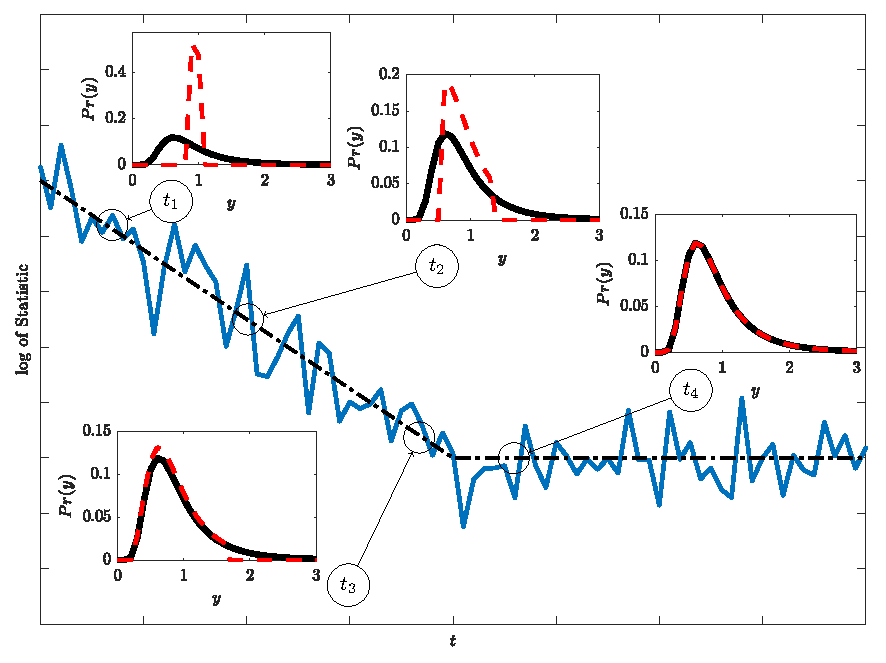
\includegraphics[width=1.0\textwidth]{figs/fig_mixing_time.pdf}
\caption{\textbf{Estimating mixing time.} The blue line shows the log of the statistical distance between the subsample and the target wealth distribution. The black dashed line is the slope of the regression line which describes the relationship between the log of the statistical distance and time, estimated separately for the mixing time period and the sable state period. The inset plots give snapshots for the empirical form of subsample distribution (red dashed line) and the target distribution at different points in time $t_1 < t_2 < t_3 < t_4$.
\label{fig:mixing-time}}
\end{figure}
\FloatBarrier

\section{Mixing time in a simple model of an economy}\label{sec:rgbm}
\subsection{Reallocating geometric Brownian motion}

To illustrate the application of mixing time in economic systems, we use Reallocating geometric Brownian motion (RGBM) as a simple model for wealth dynamics \citep{BermanPetersAdamou2019}. Under RGBM, wealth is assumed to grow multiplicatively and randomly, in addition to a simple reallocation mechanism. The dynamics of the wealth of person $i$ are specified as
%
\be
\mathrm{d} x_i = x_i \left( \mu \mathrm{d}t + \sigma \mathrm{d}W_i \right) - \tau \left( x_i - \langle x \rangle_N \right) \mathrm{d}t\,,
\label{eq:rgbm}
\ee
%
with $\mu > 0$ being the drift term, $\sigma > 0$ the fluctuations amplitude, and $\mathrm{d}W_i$ is an independent Wiener increment, $W_i(t) =\int_0^t \mathrm{d}W_i$. $\tau$ is a parameter that quantifies the reallocation of wealth. It implies that every time period $\mathrm{d}t$, everyone in the economy contributes a fraction $\tau\mathrm{d}t$ of their wealth to a central pool. The pool is then shared equally across the population ($\langle x \rangle_N$ is per-capita wealth). This parameter encapsulates multiple effects, \eg collective investment in infrastructure, education, social programs, taxation, rents paid, or private profits.

Under RGBM, the average wealth in a large population grows like $e^{\mu t}$. Rescaling by $e^{\mu t}$, the dynamic behavior of RGBM is strictly dependent on the relation between $\tau$ and $\sigma$, and the rescaled wealth can be both ergodic and non-ergodic. Since the existence of mixing is predicated on ergodic dynamics, we focus on the ergodic regime. In RGBM, rescaled wealth is ergodic when $\tau > 0$
and the model exhibits mean-reversion as each $x_i$ reverts to the population average $\langle x \rangle_N$.

The dynamics of the rescaled wealth $y_i = x_i / \langle x \rangle_N$ follow
%
\be
    \mathrm{d} y =   y \sigma  \mathrm{d} W - \tau (y - 1)  \mathrm{d}t\,,
    \label{eq:rescaled-rgbm}
\ee
%
and its stationary distribution follows (see \citep{BermanPetersAdamou2019})
%
\be
p(y) = \frac{(\beta - 1)^{\beta}}{\Gamma(\beta)} \exp{\big(-\frac{\beta - 1}{y}\big)} y^{-(1+\beta)}\,,
\label{eq:rgbm-stationary-distribution}
\ee
%
where $\beta = 1 + \frac{2 \tau}{\sigma^2}$ and $\Gamma(\cdot)$ is the Gamma function. The distribution has a power-law tail. The exponent of the power law, $\beta$, is called the Pareto tail parameter, and can be used as a measure of economic equality \citep{Cowell2011}. More importantly, important stylized facts are recovered: the larger $\sigma$ (more randomness in the dynamics) and the smaller $\tau$ (less reallocation), the smaller the tail index and the fatter the tail of the distribution, leading to higher inequality.

\subsection{Mixing time in RGBM}

A standard way for evaluating the mixing time, given a dynamical system, is by investigating the decay of correlation. In particular, a dynamical system can be said to be mixing if the autocorrelation function $\mathrm{corr(\mathrm{x}(t), \mathrm{x}(t+\delta))}$, between observations $\mathrm{x}(t)$ and $\mathrm{x}(t\delta)$, converges to $0$ as $\delta \to \infty$. The reciprocal of the rate of the decay formally gives the mixing time.

The autocorrelation function for the rescaled wealth in the ergodic regime of RGBM can be derived by performing an eigenvalue analysis of the Fokker-Planck equation, resulting in\footnote{A detailed derivation of the autocorrelation function is given in Appendix~\ref{sec:rgbm-correlation-function}.}
%
\be
\mathrm{corr(y(t), y(t+\delta))} = \exp\left[ -\tau \delta \right]\,.
\label{eq:rgbm-correlation}
\ee
%
The correlation decays in time, implying that the mixing time in RGBM is $1/\tau$. The interpretation behind this result is fairly intuitive -- in an economy in which reallocation from the rich to the poor is stronger, mixing is faster. On the other hand, as the reallocation rate approaches zero, mixing times get longer, and mobility lower.

The mixing time in RGBM can also be estimated using the estimation procedure described above. If a subsample of the population is considered, its distribution will converge to the steady state distribution of the whole population (when $\tau > 0$). The reciprocal of the convergence rate is the mixing time (see \fref{mixing-time}), and will also be equal to $1/\tau$.

\subsection{Mixing time and standard measures of mobility}\label{sec:measures}

In RGBM, unlike the mixing time, standard measures of mobility depend on the noise amplitude $\sigma$, and not only on $\tau$. This is a consequence of the randomness playing a significant role in the wealth dynamics when we consider time frames that are shorter than the mixing time. In what follows we describe the relationship between mixing time and the standard measures of mobility in RGBM.

\paragraph{Spearman's rank correlation:} Spearman's rank correlation is inversely related to the mixing time in RGBM. The rank correlation is also dependent on the noise amplitude $\sigma$ and the temporal difference $\delta$ between the two periods that are being compared. Larger values for both parameters lead to a greater economic mobility. This can be seen in~\fref{rgbm-standard-measures}A, where we plot the additive inverse of log of the rank correlation divided by $\delta$ as a function of $\tau$ for various noise amplitudes.

\begin{figure}[!htb]
\centering
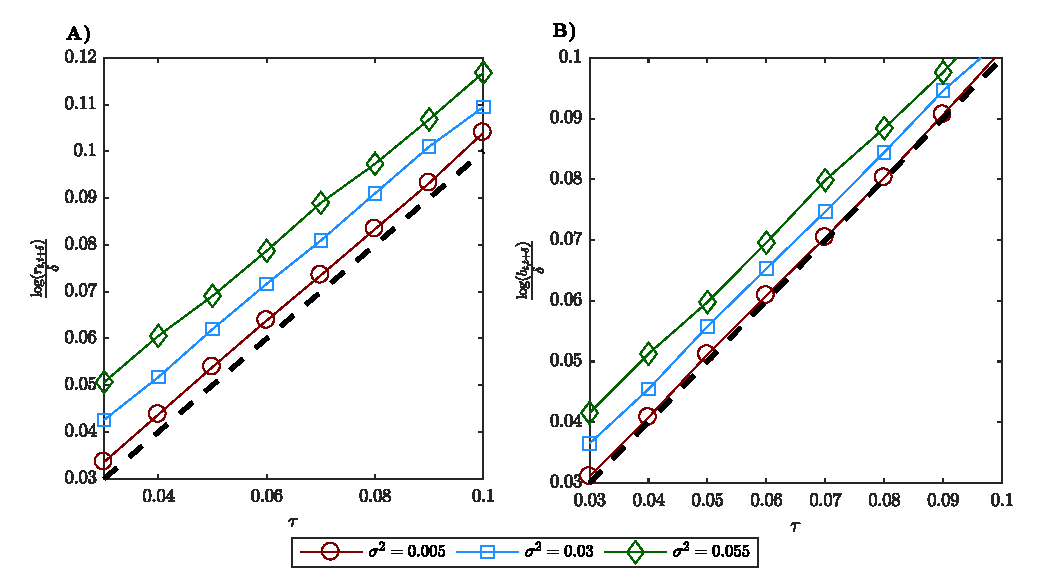
\includegraphics[width=1.0\textwidth]{figs/fig_rgbm_standard_measures.eps}
\caption{\textbf{Mixing time and standard measures of economic mobility.} \textbf{A)} Log of the Spearman's rank correlation divided by the temporal difference as a function of $\tau$. \textbf{B)} Same as \textbf{A)}, only on the y axis is the log of the IGE. The simulations used $\delta = 20$ years and $N = 10^4$ people.
\label{fig:rgbm-standard-measures}}
\end{figure}

\paragraph{Intragenerational earnings elasticity:} Similarly to the properties of the rank correlation and as evidenced in~\fref{rgbm-standard-measures}B, the IGE depends on both the noise amplitude and the magnitude of reallocation.

%\textcolor{red}{The approximate mathematical relationship between the intragenerational earnings elasticity and mixing time is studied in the Appendix.}
%In RGBM, once the dynamics reaches a stationary state, the variance of $y(t)$ is invariant on time, \ie, the variances term in equation~(\ref{eq:iee-estimation}) cancel out. Hence, the  intergenerational earnings elasticity reduces simply to the correlation between observations corresponding to two different time periods as given by equation~(\ref{eq:rgbm-correlation}). In other words, the only difference between mixing time and the intragenerational earnings elasticity is the shift in the magnitude of the later due to the dependence on the time period over which it is estimated. This finding is confirmed in Fig.~\ref{fig:rgbm-iee}, where we show the log of the stationary intragenerational earnings elasticity normalized for the time frame $\delta$ as a function of the parameter $\tau$ and vary $\sigma^2$.

\paragraph{Transition matrices:} We also consider transition (doubly stochastic) matrices $P \in \mathscr{P}\left(Q\right)$, where $p_{ij}$ represents the probability of transferring to quantile $j$ (at the end of a time period) for those starting in quantile $i$, and $Q$ is the number of quantiles. The behavior of the transition matrices follows from the properties of the previous two standard measures of mobility. In other words, it depends on both the noise amplitude and the rate of reallocation, as well as on the length of the time period in question.

As previously elaborated, the standard mobility measures describe the properties of the bivariate wealth distribution in two points in time. Such distributions are usually modeled via copulas. Mathematically, a copula can be represented by a simple model in which the transition matrix is parametrized. Widely used models are the Gaussian and the Gumbel copulas \citep{TrivediZimmer2007}. The Gaussian copula corresponds to a symmetric wealth transition matrix, whereas the Gumbel copula produces an asymmetric matrix. More precisely, under the Gumbel copula the mobility at the bottom of the distribution is higher than the mobility at the top.

A pervasive observation is that real wealth transition matrices are better modeled through the Gumbel copula exactly because of its asymmetric property \citep{JanttiJenkins2015}. Indeed, empirical studies have argued that as a consequence of this the Gaussian copula tends to underestimate the dependence in the middle of the distribution, that is, the transition probabilities between the middle quantiles \citep{BonhommeRobin2009}. 

As evidenced in~\fref{rgbm-wealth-matrices}A, the transition matrices in RGBM reproduce the asymmetric property of the real world transition matrices and are well-approximated by the Gumbel copula (\fref{rgbm-wealth-matrices}B). The major advantage of modeling through the Gumbel copula is that this copula is uniquely identified by one parameter: a larger dependence implies less mobility.

In \fref{rgbm-wealth-matrices}C we visualize the relationship between $\theta$ and the reallocation parameter $\tau$ for various noise amplitudes. We find that there is an inverse relationship between $\theta$ and $\tau$, whose slope is determined by the magnitude of $\sigma$. As $\tau$ increases, the value of the $\theta$ decreases, though disproportionately. We hereby point out that the $\theta$ parameter and the rank correlation share a direct relationship which cannot be analytically represented. As a way to visualize this relationship in \fref{rgbm-wealth-matrices}D we plot the rank correlation as a function of $\tau$.

\begin{figure}[!htb]
\centering
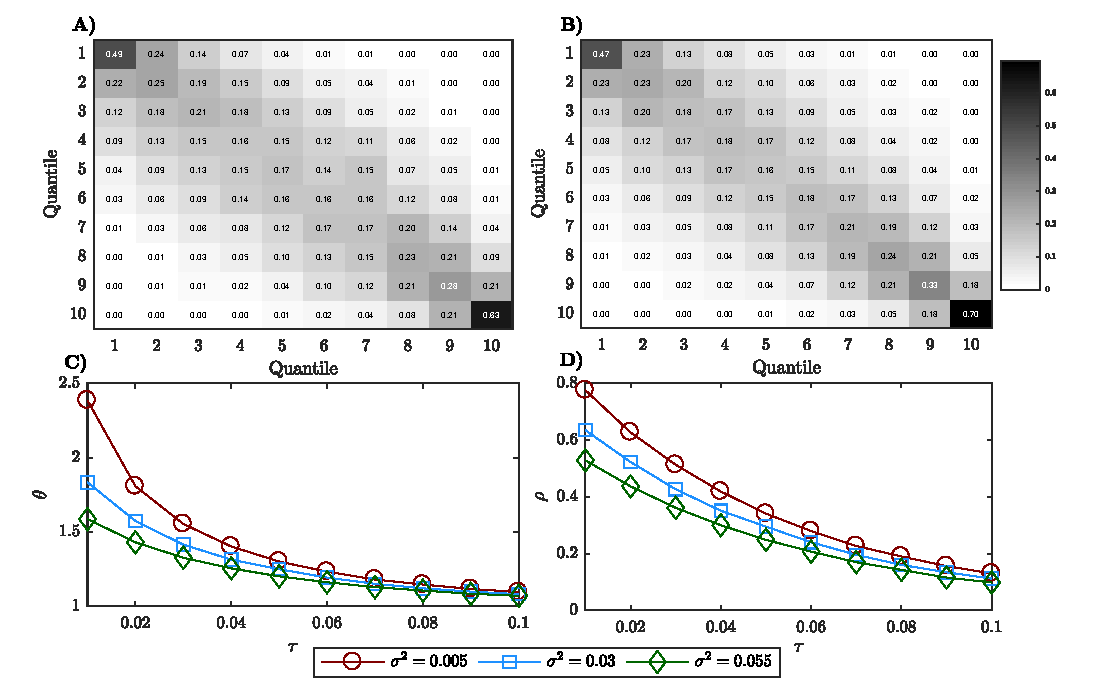
\includegraphics[width=1.0\textwidth]{figs/fig_rgbm_gumbel_v2.eps}
\caption{\textbf{Mixing time and wealth transition matrices.} \textbf{A)} Transition matrix for the stationary regime of RGBM estimated with $\tau = 0.02$ per year, $\sigma^2 = 0.01$ per year and $N = 10^4$ people. \textbf{B)} An example for a transition matrix from data simulated from a Gumbel copula whose parameter $\theta$ is chosen to be in accordance with the RGBM parameters used in \textbf{A)}. \textbf{C)} The relationship between the Gumbel copula parameter $\theta$ and the reallocation parameter $\tau$ in the stable state of RGBM. \textbf{D)} The relationship between the Gumbel copula parameter $\theta$ and the rank correlation $\rho$ in the stable state of RGBM. The parameters were estimated from a transition matrix in which $\delta = 20$ years and $N = 10^4$ people.
\label{fig:rgbm-wealth-matrices}}
\end{figure}
\FloatBarrier

\subsection{The Great Gatsby curve in RGBM}

Quantifying mobility in RGBM using mixing times allows studying the relationship between mobility and inequality. A convenient illustration of this relationship is the Great Gatsby curve, which describes an association between inequality and the intergenerational earnings elasticity across countries \citep{krueger2012,corak2013}, showing that economic \textit{immobility} and static inequality are positively related across countries.

In RGBM the mixing time, quantifying immobility, is $1/\tau$. The Pareto tail parameter is $\beta = 1 + \frac{2\tau}{\sigma^2}$ \citep{BermanPetersAdamou2019}, the inverse of which is a measure of inequality. We get that
%
\be
\frac{1}{\tau} = \frac{2}{\sigma^2\left(\beta - 1\right)}\,.
\ee
%
\fref{rgbm-great-gatsby} displays this relationship, demonstrating that RGBM reproduces the qualitative empirical observation, suggesting that inequality and immobility are positively related.

\begin{figure}[!htb]
\centering
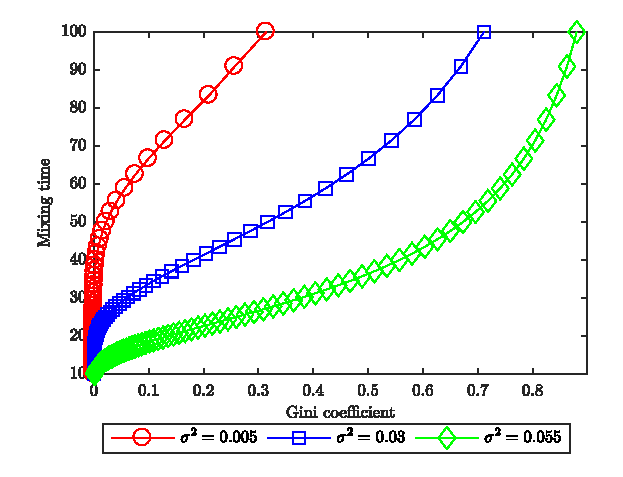
\includegraphics[width=10cm]{figs/fig_great_gatsby.eps}
\caption{\textbf{The Great Gatsby curve in RGBM.} Mixing time as a function of the inverse of the Pareto Tail coefficient in RGBM. The line colors correspond to the magnitude of the noise amplitude, as highlighted by the colormap.
\label{fig:rgbm-great-gatsby}}
\end{figure}

\FloatBarrier

\section{Discussion} \label{sec:discussion}

The existence of mobility within an economy is postulated on ergodic wealth dynamics. Thus, a measure which adequately captures the mobility within an economy should account for the possibility of non-ergodic wealth dynamics. Standard mobility measures fail to account for this property, whereas mixing time overcomes the aforementioned issues. As we showed, economic mobility will exist only when mixing time is a finite quantity, even though other measures might suggest otherwise. This is because mixing is predicated on the existence of an ergodic transformation of wealth. The ergodic transformation is characterized with a steady-state distribution and the transformed wealth distribution of any arbitrary subset of individuals belonging to the population will gradually become similar to it, if followed long enough.

Studies of wealth inequality often make the hypothesis that the ergodic transformation is given by the rescaled wealth. This case was also discussed here. However, a growing body of evidence suggests that in reality rescaled wealth might also be a non-ergodic observable. For instance, \citet{BermanPetersAdamou2019} found that, in the case of RGBM wealth dynamics, negative reallocation ($\tau < 0$) prevails in the US economy. Then, mixing time is undefined and economic mobility does not exist.
%Even in times when the reallocation was positive, the mixing time was low (between 50 and 100 years).
 
Nevertheless, another transformation of wealth might exist which is ergodic, and mixing time in terms of it will be a finite value. Then mobility exists, but can be defined in terms of an another notion. Different notions also require different analysis approaches, as they illuminate distinct extent to which mobility is socially desirable. In other words, depending on the definition of economic mobility, an increase in economic mobility will not always translate into increased economic welfare. Hence, discovering the relevant ergodic wealth transformation is extremely important for policymakers to produce adequate measures for optimizing the mobility within an economy. We refer to \citet{JanttiJenkins2015} for a lengthy discussion on the various notions of economic mobility and their social implications.

We conclude with some notes on the empirical implementation of mixing time. In general, there are two strategies that can be used to evaluate empirically the mixing time in an economy. The first one is by using the procedure described in~\Sref{mixing-time}. The main advantage of the procedure is that it offers a precise estimation of the mixing time which is independent on the assumption of wealth dynamics. However, this is an expensive procedure to perform in reality as it requires a detailed track for the wealth of a particular set of individuals. This is especially emphasized if the convergence time to the steady state distribution is slow. The second strategy requires an assumption for the wealth dynamics of each individual in the population. By combining this assumption with data on the properties of the observed wealth distribution, non-parametric methods can be implemented to infer the parameters which govern the wealth dynamics. Once the parameters are inferred, mixing time can be easily estimated via the correlation decay.  While the presented method offers an inexpensive way for quantifying mixing time, it is highly stylized in the sense that it is necessary to first assume wealth dynamics. Nonetheless, in the absence of simpler procedures, the second strategy acts as the starting point for the development of a more comprehensive methodology for estimating mixing time. We believe that with the rapid development of data gathering methods and the improved understanding of wealth dynamics within a population, some of these shortcomings will be overcome, yielding a more in-depth interpretation of mixing time in real economies.

%This paper describes the mixing time in a system of individual wealths as a measure of economic mobility. Mixing time quantifies the characteristic time for the distribution of a subsample in a population to resemble the distribution of the entire population. 
%
%It overcomes several limitations of standard statistical measures of mobility.
%
%In addition, the interpretation of the rank correlation depends on the underlying wealth distribution and its dynamics. The same rank correlation cannot be interpreted similarly when the underlying wealth distribution remains unchanged, and when it becomes more and more unequal. The IGE has similar limitations, but also others. Most notably, the IGE is sensitive by design to the level of inequality and not only to the transition matrix, as discussed in detail in the mobility literature (\eg \citet{chettyETAL2014}).
%
% This paper
%This paper introduces mixing time, a property of dynamical systems, as a measure of mobility. When wealth is an ergodic observable \citep{PetersAdamou2018c}, and assuming the wealth distribution approaches a steady state, if the wealths of an arbitrary group of individuals is followed over time, the distribution of wealth within this group will gradually become similar to the steady-state wealth distribution. The characteristic time of this process is the mixing time. Put simply, it is the time scale over which individuals mix into the wealth distribution. When mixing is rapid, \ie the mixing time is short relative to the window of observation, we could interpret that as high wealth mobility. Slow mixing is interpreted as low mobility.
%
%
%A measure which adequately captures the mobility within an economy should account for the possible non-ergodic wealth dynamics. Standard mobility measures fail to account for this property, whereas mixing time overcomes the aforementioned issues. As we showed by studying the simple model of RGBM, economic mobility will exist only when mixing time is a finite quantity, even though other measures might suggest otherwise. This is because mixing is predicated on the existence of an ergodic transformation of wealth. The ergodic transformation is characterized with a steady-state distribution and the transformed wealth distribution of any arbitrary subset of individuals belonging to the population will gradually become similar to it, if followed long enough.
%
%Studies of wealth inequality often make the hypothesis that the ergodic transformation is given by the rescaled wealth. This case was also discussed here. However, a growing body of evidence suggests that in reality rescaled wealth might also be a non-ergodic observable. Then, mixing time is undefined and economic mobility does not exist. Nevertheless, another transformation of wealth might exist which is ergodic, and mixing time in terms of it will be a finite value. Then mobility will definitely exist but it should be defined in terms of another notion \citep{JanttiJenkins2015}.
%
%In general, there are two strategies that can be used to evaluate empirically the mixing time in an economy. The first one is by using the procedure described in~\Sref{mixing-time}. The main advantage of the procedure is that it offers a precise estimation of the mixing time which is independent on the assumption of wealth dynamics. However, this is an expensive procedure to perform in reality as it requires a detailed track for the wealth of a particular set of individuals. This is especially emphasized if the convergence time to the steady state distribution is slow.
%
%The second strategy requires an assumption for the wealth dynamics of each individual in the population. By combining this assumption with data on the properties of the observed wealth distribution, non-parametric methods can be implemented to infer the parameters which govern the wealth dynamics. Once the parameters are inferred, mixing time can be easily estimated via the correlation decay. For instance, this procedure was used in \citet{BermanPetersAdamou2019} to estimate the RGBM parameters in the United States (US) economy. Their results suggest that currently in the US  negative reallocation ($\tau < 0$) prevails, thus implying that mixing time does not exist for the rescaled wealth. Even in times when the reallocation was positive, the mixing time was low (between 50 and 100 years).  
%
%While the presented method offers an inexpensive way for quantifying mixing time, it is highly stylized in the sense that it is necessary to first assume wealth dynamics. Nonetheless, in the absence of a simpler procedures, the second strategy acts as the starting point for the development of a more comprehensive methodology for estimating mixing time. We believe that with the rapid development of data gathering methods and the improved understanding of wealth dynamics within a population, some of these shortcomings will be overcome, yielding a more in-depth interpretation of mixing time in real economies.

%\bibliography{../LML_bibliography/bibliography}
\bibliography{mixing-time}
\clearpage

\appendix

\section{Definitions of standard mobility measures}\label{sec:standard-mobility-measures}

\paragraph{Spearman's rank correlation:} Spearman's rank correlation is defined on a joint distribution of wealth at two points in time, $t_m$ and $t_n$ ($t_m < t_n$). It is defined as
%
\be
    r_{t_m,t_n} = 1 - \frac{6\sum_i \left[rg\left(\mathrm{x}_i\left(t_m\right)\right) - rg\left(\mathrm{x}_i\left(t_n\right)\right)\right]^2}{N\left(N^2-1\right)}\,,
\ee
%
where $rg(\mathrm{x})$ is the rank transformation of $\mathrm{x}$, $\mathrm{x}_i(t)$ is the wealth of individual $i$ in period $t$ and $N$ is the population size. This measure is bounded between $-1$ and $1$. $r_{t_m,t_n} = 1$ suggests perfect immobility, a state in which there is no change in wealth ranks between the two points in time. Lower values suggest greater economic mobility.

\paragraph{Intragenerational earnings elasticity:} The intragenerational earnings elasticity is defined as the slope $b_{t_m,t_n}$ of the regression
%
\be
   \log\left(\mathrm{x}_i\left(t_n\right)\right) = b_0 + b_{t_m,t_n} \log\left(\mathrm{x}_i\left(t_m\right)\right) + u_i\,,
\ee
%
where $b_0$ is the intercept and $u_i$ is the error term. This is a simple linear regression and therefore,
%
\be
    b_{t_m,t_n} = \mathrm{corr}\left(\log\left(\mathrm{x}\left(t_n\right)\right),\log\left(\mathrm{x}\left(t_m\right)\right)\right) \frac{\mathrm{var}\left(\log\left(\mathrm{x}\left(t_n\right)\right)\right)}{\mathrm{var}\left(\log\left(\mathrm{x}\left(t_m\right)\right)\right)}\,,
    \label{eq:iee-estimation}
\ee
%
where $\mathrm{corr}(\mathrm{x},\mathrm{y})$ is the correlation between the variables $\mathrm{x}$ and $\mathrm{y}$ and $\mathrm{var}(\mathrm{x})$ is the variance of $\mathrm{x}$. As with the rank correlation, lower IGE also indicates greater mobility. However, this measure is unbounded and may take on any real values.

\paragraph{Wealth transition matrix:} The wealth transition matrix disaggregates wealth rankings and summarizes economic mobility in a
transition matrix $\mathbf{A}$ in which the elements $A_{kl}$ quantify the probability that an individual in wealth quantile $k$ in period $t_m$ is found in wealth quantile $l$ in period $t_n$. In a perfectly mobile economy, the entries of the transition matrix are all equal to each other. This would correspond to $0$ rank correlation. In an immobile economy, on the other hand, the largest values are concentrated in the diagonal entries. A perfectly immobile case, of rank correlation $1$, would correspond to the identity transition matrix.

\section{Numerical presentation of Mixing time}\label{sec:rgbm-numerical-mixing-time}

We use RGBM to numerically present the procedure described in~\Sref{mixing-time}. In the concrete example, we focus on the role of the subsample size, $\tau$ and $\sigma$ in the duration of the mixing time period and the estimation of the mixing time measure. 

For this purpose, in~\Fref{rgbm-mixing-time}A-B we plot the log of Kolmogorov-Smirnov (KS) statistic as a function time and vary the subsample size, reallocation rate and the noise amplitude. Intuitively, the reallocation rate uniquely determines the mixing time, whereas the noise amplitude has no effect, as argued in~\Sref{rgbm}. However, it appears that the subsample size critically determines the behavior of the stable state in the system as it determines the value of the stationary KS statistic (\Fref{rgbm-mixing-time}C). This is because the estimation of the KS statistic relies on the differences between the empirical distribution function and the cumulative distribution function for the target stationary wealth distribution. Due to the subsample size always being a finite number, in empirical calculations, there will be differences between the empirical distribution and the target distribution, which will be translated in a positive KS statistic. As the subsample size increases, in the limit as the subsample size goes towards infinity, the differences will disappear.

\begin{figure}[!htb]
\centering
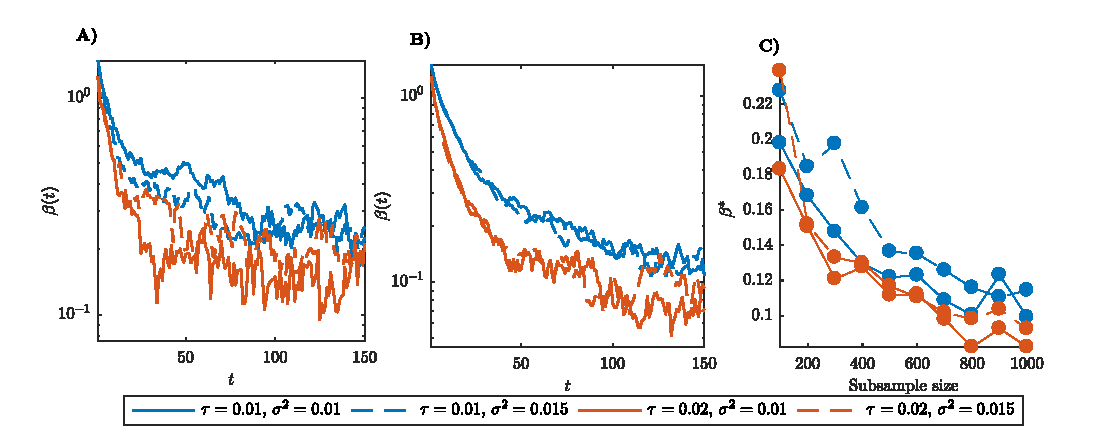
\includegraphics[width=1.0\textwidth]{figs/fig_mixing_time_rgbm.eps}
\caption{\textbf{Mixing time in RGBM.} \textbf{A)} Log of KS statistic as a function of time for a realization of an RGBM process with a subsample size of $10^4$ for different noise amplitudes and reallocation parameters. \textbf{B)} Same as \textbf{A)}, only with a subsample size of $10^5$ people. \textbf{C)} The log of the stationary KS statistic as a function of the subsample size for various $\sigma^2$ and $\tau$. In the simulations $N = 10^6$ people. \label{fig:rgbm-mixing-time}}
\end{figure}

\section{Derivation of the correlation function in RGBM}\label{sec:rgbm-correlation-function}

The autocorrelation function $\mathrm{corr}(\mathrm{x}(t), \mathrm{x}(t+\delta))$ of a stochastic process is simply the Pearson correlation between observables of the process corresponding to two different time points $t$ and $t+\delta$, 
\be
    \mathrm{corr}(\mathrm{x}(t), \mathrm{x}(t+\delta)) = \frac{\mathrm{cov}(\mathrm{x}(t), \mathrm{x}(t+\delta))}{\sqrt{\mathrm{var}(\mathrm{x}(t))} \sqrt{\mathrm{var}(\mathrm{x}(t+\delta))}},
    \label{eq:autocorrelation}
\ee
where $\mathrm{cov}(\mathrm{x}, \mathrm{y})$ is the covariance between $\mathrm{x}$ and $\mathrm{y}$.

Eq.~\eqref{eq:rgbm-correlation} gives the autocorrelation in the stationary regime of RGBM, that is, when $t \to \infty$. In this case the variance of the process corresponding to different time points is the same. Thus, for the denominator of~\eqref{eq:autocorrelation} in RGBM we have,
\be
   \sqrt{\mathrm{var}(y(t))} \sqrt{\mathrm{var}(y(t+\delta))} = \mathrm{var(y(t))} = \mathrm{var(y(t+\delta))} = \frac{\sigma^2}{2\tau - \sigma^2}.
    \label{eq:rgbm-variance}
\ee
The right hand side of Eq.~\eqref{eq:rgbm-variance} can be easily derived using Ito calculus (see \citet{BermanPetersAdamou2019}).

The derivation of the autocovariance function present in the numerator of~\eqref{eq:rgbm-correlation} is a bit more tricky. A standard way for estimating such functions is by utilizing the eigenfunctions $\psi(\lambda,\mathrm{x})$ and eigenvalues $\lambda$ of the Fokker-Planck equation corresponding to the stochastic process. Once, they are inferred, the autocovariance function can be found as
\be
\mathrm{cov}(\mathrm{x}(t), \mathrm{x}(t+\delta)) = \sum_n g_n^2 \exp\left[ -\lambda_n \delta \right] + \int g(\lambda)\exp\left[ -\lambda \delta \right],
\label{eq:covariance-stochastic-process}
\ee
where with the subscript $n$ we denote the discrete spectrum of the system, and
\be
g = \int \mathrm{x} \psi(\lambda,\mathrm{x}) d\mathrm{x}.
\ee
In RGBM, it turns out that all $g$'s are 0, except the one corresponding to the first eigenvalue of the discrete spectrum. The value of this eigenvalue is simply $\tau$ and the corresponding eigenfunction is \citep{LiuSerota2017}
%
\be
\psi_1(\lambda_1,y) = \frac{\exp\left[\frac{-2\tau}{\sigma^2 y}\right](y-1) (\frac{2\tau}{y \sigma^2})^{2+\frac{2\tau}{\sigma^2}}}{(\frac{2\tau}{\sigma^2})^2\sqrt{\Gamma (\frac{2\tau}{\sigma^2}) \Gamma (\frac{2\tau}{\sigma^2}-1})}.
\label{eq:eigenfunction-rgbm}
\ee
This results in
\be
g_1 = \frac{1}{\sqrt{\frac{2\tau}{\sigma^2}-1}}.
\label{eq:g-rgbm}
\ee
Combining~\eqref{eq:g-rgbm} with~\ref{eq:covariance-stochastic-process} we get that the covariance in RGBM is
\be
\mathrm{cov}(y(t), t(t+\delta)) = \frac{\exp\left[-\tau \delta\right]}{\frac{2\tau}{\sigma^2}-1}.
\label{eq:rgbm-covariance}
\ee
Inserting~\eqref{eq:rgbm-variance} and~\eqref{eq:rgbm-covariance} we recover the RGBM correlation function~\eqref{eq:rgbm-correlation}.

\section{Properties of standard mobility measures in RGBM}\label{sec:properties-standard-mobility-measures}

In this section we investigate in greater detail the relationship between $\sigma$ and $\delta$ and the standard measures of economic mobility in the ergodic regime of RGBM. For this reason we conduct two numerical experiments where we explore the stationary behavior of the rank correlation and IGE. 

In the first experiment, we study the association between the standard measures of mobility and the noise amplitude $\sigma$. \Fref{rgbm-standard-measures-sigma} gives the results. From \Fref{rgbm-standard-measures-sigma}A-B we infer that that the rank correlation and IGE are approximately linearly related with $\sigma^2/2$ when they are, respectively, transformed as $-\tau - \frac{\log(\rho(t,t+\delta))}{\delta}$ and $-\tau - \frac{\log(b_{(t,t+\delta))}}{\delta}$. The marginal effect of $\tau$ on the slope of the relationship is shown in \Fref{rgbm-standard-measures-sigma}C. Obviously, as $\tau$ increases the slope decreases linearly.

\begin{figure}[!htb]
\centering
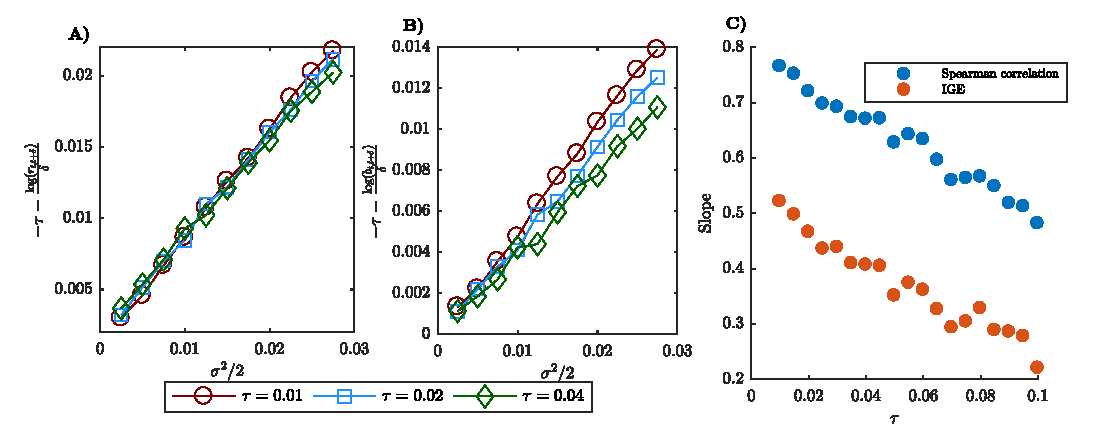
\includegraphics[width=1.0\textwidth]{figs/fig_rgbm_sigma_relationship.eps}
\caption{\textbf{Relationship between the noise amplitude and standard measures of economic mobility.} \textbf{A)} Difference between $-\tau$ and the log of the Spearman's rank correlation divided by the temporal difference as a function of $\sigma^2/2$. \textbf{B)} Same as \textbf{A)}, only on the y axis is the difference between $-\tau$ and the log of the IGE. \textbf{C)} Slope of the lines presented in \textbf{A-B}, as a function of $\tau$. 
\textbf{A-C} In the simulations, $\delta = 20$ years and $N = 10^4$ people.
\label{fig:rgbm-standard-measures-sigma}}
\end{figure}
\FloatBarrier

In the same same fashion, in \Fref{rgbm-standard-measures-delta} we examine the effect of the magnitude of the temporal difference on the rank correlation and the IGE. As indicated in \Fref{rgbm-standard-measures-delta}, $\delta$ is approximately linearly related with the rank correlation and IGE when their transformations are $\frac{-\log(\rho(t,t+\delta))}{\tau + \frac{\sigma^2}{2}}$ and $\frac{\log(b_{(t,t+\delta))}}{\delta}$. In this case, increments in the reallocation parameter have a positive impact on the slope of the relationship.

\begin{figure}[!htb]
\centering
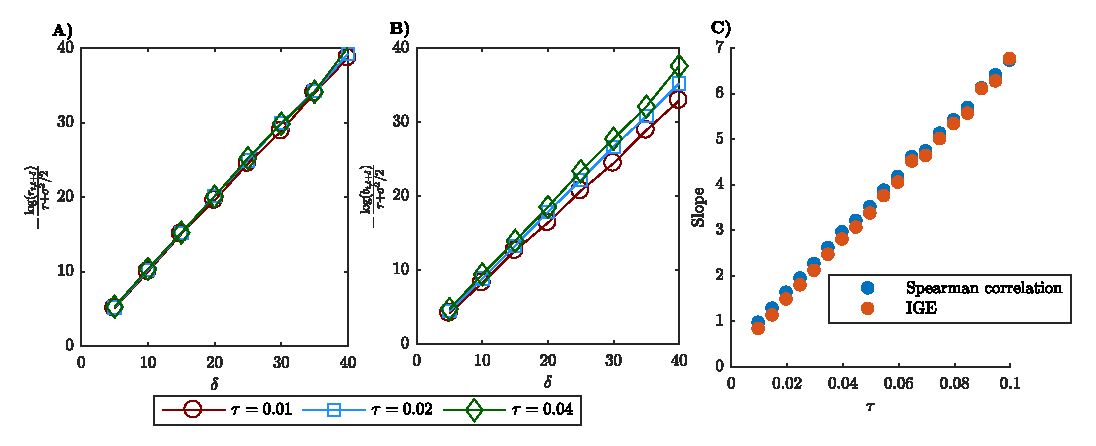
\includegraphics[width=1.0\textwidth]{figs/fig_rgbm_delta_relationship.eps}
\caption{\textbf{Relationship between the temporal difference and standard measures of economic mobility.} \textbf{A)} Additive inverse of the logarithm of the rank correlation divided by $\tau +\frac{\sigma^2}{2}$ as a function of $\delta$. \textbf{B)} Same as \textbf{A)}, only on the y axis only for the logarithm of IGE. \textbf{C)} Slope of the lines presented in \textbf{A-B}, as a function of $\tau$. 
\textbf{A-C} In the simulations, $\delta = 20$ years and $N = 10^4$ people.
\label{fig:rgbm-standard-measures-delta}}
\end{figure}
\FloatBarrier

\end{document}

%% THIS SECTION IS OUT OF THE DOCUMENT AND IT IS NOT NEEDED FOR NOW
\section{Derivation of IEE in RGBM}

As a measure, the intergenerational earnings elasticity is determined by the dynamics of the log of (rescaled) wealth $z = \log(y)$. Using Ito calculus, we can recover the following equation for the dynamics of $z$,
\begin{align*}
    d z &= \tau \bigg( \exp(-z) - \frac{2\tau + \sigma^2}{2 \tau} \bigg) dt + \sigma dW.
\end{align*}
The stationary distribution of the process can be found by using the transformation law of probabilities, 
\begin{align}
    P_z(z) &= P_y\big(\exp(z)\big) \exp(z).
\end{align}
The first and second moment of this distribution are
\begin{align}
\langle z \rangle &= -\psi(\theta) + \log(\theta - 1), \\
\langle z^2 \rangle &= \psi^{(1)}(\theta) + \bigg( \psi^{(1)}(\theta) - \log(\theta-1)\bigg)^2.
\end{align}
See \citet{DutreDebosscher1977,Debosscher1990} for the derivation of the transitory PDF of both $y$ and $z$.
